\\ \textbf{Question 12.} \\
\hrule 

Consider randomly selecting a student at a large university, and let $A$ be the event that the selected student has a Visa card and $B$ be the analogous event for MasterCard. Suppose that $P(A) = .6$ and $P(B) = .4$.

\textbf{a. Could it be the case that $P(A \cap B) = .5$? Why or why not?}
It cannot be the case. The intersection of the two events cannot possibly be greater than the value of one of the individual events. The highest $P(A \cap B)$ could be is 0.4, and that is only if $B$ completely intersected with $A$.

\textbf{b. From now on, suppose that $P(A \cap B) = .3$. What is the probability that the selected student has at least one of these two types of cards? } \newline 
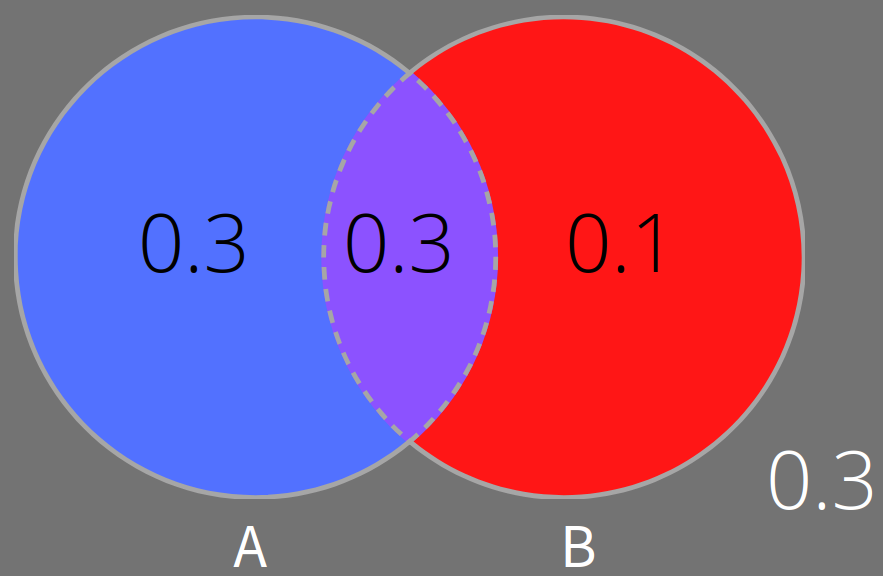
\includegraphics[scale=0.25]{images/whw3/2.2.12_venn.png}

The probability of this can be found by simply adding up the three probabilities within the circles. That would give us $P(A \cup B) = .7$

\textbf{c. What is the probability that the selected student has neither type of card.} \newline 
This one can be found by simply subtracting the .7 we just got from 1. If a student doesn't have at least one of the two cards, then they have neither. Simple as that. This can be represented as $P(A' \cap B') = .3$.

\textbf{d. Describe, in terms of $A$ and $B$, the event that the selected student has a Visa card but not a MasterCard, and then calculate the probability of the event.} \newline
This can be described as the blue circle minus the intersecting part in the middle. We can describe that as $P(A \cap B') = .3$. We know the value is .3 because the intersection between the two events is .3, and $.6 - .3 = .3$.

\textbf{e. Calculate the probability that the selected student has exactly one of the two types of cards.} \newline
This one is easy. We simply add the two outer circles together and ignore the intersection. As such, that gives us $P((A \cup B) - A \cap B) = .4$